\chapter{Konfigurieren des TransistorTesters}
\label{sec:config}
Die ganze Software des TransistorTesters ist im Quellcode verf\"ugbar.
Die "Ubersetzung der Module wird mit einer Makefile gesteuert. Die Entwicklung wurde
auf einen Ubuntu Linux Betriebssystem mit den GNU Werkzeugen (GNU toolchain, gcc version 4.5.3) durchgef\"uhrt.
Es sollte m\"oglich sein, ohne Schwierigkeiten andere Linux Betriebssysteme zu benutzen.
Um die \"ubersetzen Daten in den Flash-Speicher oder den EEprom Speicher zu laden, wird das
Programm avrdude (Version 5.11svn) von der Makefile benutzt, wenn man ,,make upload'' aufruft.
Das Programm avrdude ist f\"ur Linux und Windows Betriebssysteme verf\"ugbar.
Der GNU C-Kompiler wird auch von der AVR studio Software unter Windows benutzt.
Sie k\"onnen die Programm Daten (.hex und .eep) auch mit anderen Programmen in den ATmega laden,
aber nur meine Makefile Version stellt sicher, da"s die richtigen Daten in den gew\"ahlten Prozessor gelangen.
Avrdude l\"ad Daten nur in den ATmega, wenn die Signatur Bytes des angeschlossenen ATmega gleich mit dem ausgew\"ahlten sind.
Wenn Sie die Makefile \"andern, wird die Software komplett neu \"ubersetzt, wenn man ,,make'' oder
,,make upload'' aufruft.
Die Software, die f\"ur einen ATmega8 \"ubersetzt wurde, l\"auft nicht auf einem ATmega88.
Die Software, die f\"ur einen ATmega168 \"ubersetzt wurde, l\"auft nicht auf einem ATmega88, sogar wenn
der ATmega88 genug Speicher hat!
Sind Sie vorsichtig, wenn Sie nicht meine Makefile benutzen.
Mit den entsprechenden Optionen ist die Software auch auf dem unver\"anderten Hardware-Entwurf von
Markus F. lauff\"ahig (PARTNO=m8 , keine NO\_AREF\_CAP und keine PULLUP\_DISABLE Option).
Die Taktrate kann mit den fuses auch auf 8MHz gestellt werden, dazu ist kein Quarz erforderlich!


Die folgenden Optionen der Makefile sind verf\"ugbar, um die Software f\"ur den Tester zu konfigurieren:

\begin{description}
  \item[PARTNO] beschreibt den Ziel-Prozessor:\\
         m8 = ATmega8\\
         m88 or m88p = ATmega88\\
         m168 or m168p = ATmega168\\
         m328 or m328p = ATmega328\\
    Beispiel:  PARTNO = m168
  \item[UI\_LANGUAGE] gibt die Sprache f\"ur den Tester an\\
    LANG\_ENGLISH, LANG\_GERMAN, LANG\_POLISH, LANG\_CZECH,  LANG\_SLOVAK und  LANG\_SLOVENE sind derzeit verf\"ugbar.\\
    Beispiel: UI\_LANGUAGE = LANG\_ENGLISH
  \item[LCD\_CYRILLIC] wird nur gebraucht, wenn man ein LCD-Display mit kyrillischem Zeichensatz benutzt.
Das \(\mu\) und \(\Omega\) Zeichen ist im kyrillischen Zeichensatz nicht enthalten.
Wenn Sie diese Option angeben, werden beide Zeichen von der Software in das LCD geladen.\\
Beispiel: CFLAGS += -DLCD\_CYRILLIC
  \item[WITH\_SELFTEST] Wenn Sie diese Option angeben, baut die Software eine Selbsttest-Funktion ein, die gestartet wird
wenn Sie alle drei Pr\"ufspitzen verbinden und eine Messung starten.\\
Beispiel: CFLAGS += -DWITH\_SELFTEST
  \item[AUTO\_CAL] Der Nullabgleich f\"ur die Kondensatormessung und der Innenwiderstand der Port-Ausg\"ange wird beim
Selbsttest zus\"atzlich ins EEprom geschrieben und ist damit f\"ur die weiteren Messungen abgeglichen.
Wenn nach dem Nullabgleich der Kondensatormessung ein Kondensator mit einer Kapazit\"at zwischen \(100 nF\) und \(20 \mu F\) an Pin~1 und Pin~3 
angeschlossen wird, wird auch der Offset des analogen Komparators und die Skalierung f\"ur die AUTOSCALE\_ADC
Umschaltung auf die interne Spannungsreferenz ermittelt und ins EEprom geschrieben.\\
Beispiel: CFLAGS += -DAUTO\_CAL
  \item[FREQUENCY\_50HZ] Zum Ende des Selbsttests wird bis zu einer Minute lang ein 50 Hz Signal auf Port 2 und Port 3 erzeugt.\\
Beispiel: CFLAGS += -DFREQUENCY\_50HZ
  \item[R\_MESS] schaltet die Widerstandsmessung ein.
 Diese Option sollte immer angegeben werden.\\
Beispiel: CFLAGS += -DR\_MESS
  \item[C\_MESS] schaltet die Kondensatormessung ein.
 Diese Option sollte immer angegeben werden.\\
  \item[CAP\_EMPTY\_LEVEL] Diese Option legt die Spannung (mV) f\"ur einen entladenen Kondensator fest.
Der Wert kann h\"oher als 3mV gesetzt werden, wenn die Entladung nicht zum Ende kommt. In diesen Fall meldet der Tester nach l\"angerer Zeit ,,Cell!''.\\
Beispiel: CFLAGS += -DCAP\_EMPTY\_LEVEL=3
  \item[WITH\_AUTO\_REF] Mit dieser Option wird die Referenzspannung gemessen, um den aktuellen Faktor f\"ur die Kapazit\"atsmessung 
von kleinen Kapazit\"aten (unter \(40\mu F\)) zu ermitteln.\\
Beispiel:  CFLAGS += -DWITH\_AUTO\_REF
  \item[REF\_C\_KORR] gibt einen Offset f\"ur die gelesene Referenz-Spannung in mV Einheiten an.
Das kann benutzt werden um die Kapazit\"atsmessung kleiner Kondensatoren abzugleichen.
Wenn zus\"atzlich die AUTO\_CAL Option gew\"ahlt wurde, ist diese Angabe nur ein zus\"atzlicher Offset f\"ur
den gefundenen Komparator-Offset.
Ein Wert von 10 ergibt etwa 1~Prozent kleinere Me"sergebnisse.\\
Beispiel:  CFLAGS += -DREF\_C\_KORR=14
  \item[C\_H\_KORR] gibt eine Korrektur der Me"sergebnisse f\"ur gro"se Kondensatoren an.
Eine Eingabe von 10 f\"uhrt zu 1~Prozent kleineren Me"sergebnissen.\\
Beispiel:  CFLAGS += -DC\_H\_KORR=10
  \item[AUTOSCALE\_ADC] schaltet die automatische Bereichswahl des ADC (entweder VCC oder interne Referenz) ein.
Die interne Referenz hat 2,56V f\"ur den ATmega8 und 1,1V f\"ur die anderen Prozessoren.\\
Beispiel: CFLAGS += -DAUTOSCALE\_ADC
  \item[ESR\_ZERO] gibt einen Nullwert f\"ur die ESR Messung von Kondensatoren vor. Dieser Nullwert wird von den
ermittelten Me"swerten abgezogen. Bei negativen ESR-Werten wird die Ausgabe ,,ESR=?'' angezeigt und der Nullwert
im EEprom korrigiert. Dieser korrigierte Wert wird bei den folgenden Messungen wirksam.
Falls Sie immer zu hohe ESR-Werte messen, sollten Sie diesen Vorgabewert erh\"ohen.\\
Beispiel: CFLAGS += -DESR\_ZERO=29
  \item[NO\_AREF\_CAP] teilt der Software mit, da"s Sie keinen Kondensator am AREF Pin (Pin 21) angeschlossen haben.
Dies erm\"oglicht k\"urzere Wartezeiten f\"ur die AUTOSCALE\_ADC Umschaltung des ADC.
Ein 1nF Kondensator wurde in diesem Modus ohne Fehler getestet.
Die Abbildungen~\ref{pic:aref1} und \ref{pic:aref5} zeigen die Schaltzeiten mit einem 1nF Kondensator.
Wie Sie sehen k\"onnen ist das Schalten von 5V auf 1,1V viel langsamer als das Zur\"uckschalten auf 5V.
Wenn Sie noch einen \(100 nF\) installiert haben, ist die Schaltzeit etwa Faktor 100 l\"anger!\\
Beispiel: CFLAGS += -DNO\_AREF\_CAP
  \item[REF\_R\_KORR] gibt einen Offset f\"ur die interne Referenz-Spannung in mV Einheiten an.
Mit diesem Offset kann eine Differenz bei der Umschaltung der Referenzspannung f\"ur die Widerstandsmessung abgeglichen werden.
Wenn die AUTO\_CAL Option gew\"ahlt wurde, ist dieser Wert nur ein Offset zu der gefundenen Spannungs-Differenz in der
AUTO\_CAL Funktion.\\
Beispiel:  CFLAGS += -DREF\_R\_KORR=10
  \item[OP\_MHZ] gibt der Software an, mit welcher Taktfrequenz in MHz der Tester arbeiten wird.
Die Software ist nur mit 1MHz, 8MHz und zus\"atzlich auch 16MHz getestet. Der 8MHz Betrieb wird wegen der besseren Aufl\"osung der
Kondensator- und Spulen-Messung empfohlen.\\
Beispiel: OP\_MHZ = 8
  \item[USE\_EEPROM] gibt an, ob feste Texte und Tabellen im EEprom Speicher abgelegt werden sollen.
Anderenfalls wird der Programmspeicher (flash) benutzt.
Es wird empfohlen, den EEprom Speicher zu benutzen (Option gesetzt).\\
Beispiel: CFLAGS += -DUSE\_EEPROM
  \item[PULLUP\_DISABLE] gibt an, da"s man die internen ,,pull-up'' Widerst\"ande nicht ben\"otigt.
 Sie m\"ussen einen externen ,,pull-up'' Widerstand an Pin 13 (PD7) und VCC angeschlossen haben, um diese
Option benutzen zu k\"onnen.
Mit dieser Option wird ein m\"oglicher Einflu"s der ,,pull-up'' Widerst\"ande auf die Me"s-Ports (Port B und Port C) verhindert.\\
Beispiel: CFLAGS += -DPULLUP\_DISABLE
  \item[ANZ\_MESS] diese Option gibt an, wie oft der ADC-Wert eingelesen und addiert werden soll.
Sie k\"onnen einen Wert zwischen 5 und 200 w\"ahlen um einen Mittelwert f\"ur eine ADC Messung zu bilden.
H\"ohere Werte ergeben eine bessere Genauigkeit, aber brauchen l\"angere Me"szeit.
Eine ADC-Messung mit dem Wert 44 braucht etwa 5ms.\\
Beispiel: CFLAGS += -DANZ\_MESS=44
  \item[POWER\_OFF] Diese Option schaltet die automatische Abschaltfunktion ein.
Wenn Sie diese Option weglassen, werden die Messungen in einer Schleife endlos wiederholt, bis die Betriebs-Spannung 
unterbrochen wird (Ein/Aus Schalter).
Wenn Sie einen Tester ohne die Schalttransistoren haben, k\"onnen Sie diese Option weglassen.
Wenn Sie mit den installierten Schalttransistoren die Option POWER\_OFF weggelassen haben,
k\"onnen Sie die Mess-Wiederholung dennoch abbrechen, wenn Sie den Start-Knopf einige Sekunden ged\"uckt halten 
w"ahrend das Me"sergebnis angezeigt wird bis die ,,Timeout'' Meldung erscheint.
Wenn Sie den Knopf loslassen, schaltet der Tester den Strom ab.
Sie k\"onnen auch angeben, nach wie vielen Messungen ohne gefundenes Bauteil der Tester ausschaltet.
Bei doppelt so viel aufeinanderfolgenden Messungen mit gefundenem Bauteil schaltet der Tester auch ab,
wenn nicht zwischendurch eine Messung ohne gefundenes Bauteil war.
Wenn Sie vergessen haben, ein angeschlossenes Bauteil abzuklemmen, wird so eine vollst\"andige Batterie-Entladung
verhindert.
Bei einer Options-Angabe in der Form von CFLAGS += -DPOWER\_OFF=5 wird nach 5 aufeinanderfolgenden Messungen ohne
gefundenes Bauteil abschaltet. Aufeinanderfolgende 10 Messungen mit gefundenem Bauteil schalten ebenfalls aus.
Nur wenn die jeweilige Me"s-Serie durch den anderen Typ unterbrochen wird, wird die Messung fortgesetzt.
Die Me"sresultate f\"ur eine Einzelmessung werden 10~Sekunden angezeigt, bei der Mehrfachmessung wird die
Anzeigezeit auf 3~Sekunden reduziert (wird in config.h gesetzt).
Wenn der Startknopf beim ersten Einschalten lange gedr\"uckt wird, wird das Me"sergebnis
 auch bei der Mehrfachmessung 10~Sekunden angezeigt.
Der Maximalwert f\"ur die Wiederholungen ist 255 (CFLAGS += -DPOWER\_OFF=255).\\
Beispiel 1: CFLAGS += -DPOWER\_OFF=5 \\
Beispiel 2: CFLAGS += -DPOWER\_OFF 
  \item[BAT\_CHECK] schaltet die Batterie Spannungspr\"ufung ein.
 Wenn Sie diese Option nicht angeben, wird die Versions-Nummer der Software angezeigt.
Diese Option ist hilfreich um bei Batterie betriebenen Tester Versionen an den Batterie Wechsel zu erinnern.\\
Beispiel: CFLAGS += -DBAT\_CHECK
  \item[BAT\_OUT] schaltet die Batterie Spannungsanzeige auf dem LCD ein, wenn BAT\_CHECK gew\"ahlt wurde.
 Wenn Ihre 9V Versorgung eine Diode wegen des Verpolungs-Schutzes installiert hat, k\"onnen Sie 
die Form BAT\_OUT=600 angeben, um die Dioden-Schwellspannung 
bei der Spannungsanzeige zu ber\"ucksichtigen.
Auch der Spannungsverlust am Transistor T3 kann so mit dieser Option ber\"ucksichtigt werden.
Die Angabe der Schwellspannung in mV beeinflu"st nicht die Pr\"uf\-span\-nungs Werte (BAT\_POOR).\\
Beispiel 1: CFLAGS += -DBAT\_OUT=300 \\
Beispiel 2: CFLAGS += -DBAT\_OUT
  \item[BAT\_POOR] setzt die Leer-Spannung f\"ur die Batteriespannungs-Pr\"ufung auf den angegebenen 100mV (0,1V) Wert.
Die Warn-Spannung ist immer 1V h\"oher als die angegebene Leer-Spannung.
Das Setzen der Leer-Spannung auf Werte wie 5,4V wird f\"ur wiederaufladbare 9V Batterien nicht empfohlen,
weil das die Gefahr von Batterie-Sch\"aden wegen der Tief-Entladung erh\"oht!
Wenn Sie wiederaufladbare 9V Batterien einsetzen, werden ,,Ready to Use'' Typen wegen der geringeren Selbstentladung empfohlen.\\
Beispiel f\"ur low drop Regler (5.4V): CFLAGS += -DBAT\_POOR=54 \\
Beispiel f\"ur 7805 type Regler (6.4V): CFLAGS += -DBAT\_POOR=64
  \item[PROGRAMMER] stellt den Programmer Typ f\"ur das avrdude Schnittstellenprogramm ein.
Eine richtige Einstellung des Programmer Typs (und Ports) ist notwendig, wenn Sie den ,,make upload'' oder
,,make fuses'' Aufruf dieser Makefile benutzen.
F\"ur weitere Informationen schauen Sie bitte in die Handbuch Seiten von avrdude oder in die online Dokumentation~\cite{avrdude}.\\
Beispiel: PROGRAMMER=avrisp2
  \item[PORT] stellt die verwendete Schnittstelle ein, wo avrdude den Mikrocontroller (ATmega) erreichen kann.
F\"ur weitere Informationen schauen Sie bitte in die Handbuch Seiten von avrdude.\\
Beispiel: PORT=usb

\end{description}

\begin{figure}[H]
  \begin{subfigure}[b]{9cm}
    \centering
    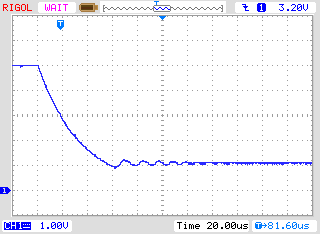
\includegraphics[width=9cm]{../PNG/AREF2_1V.png}
    \caption{from 5V to 1.1V }
    \label{pic:aref1}
  \end{subfigure}
  ~
  \begin{subfigure}[b]{9cm}
    \centering
    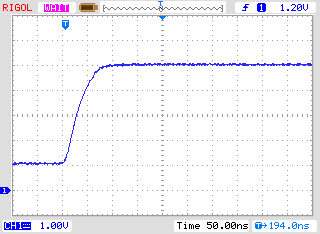
\includegraphics[width=9cm]{../PNG/AREF2VCC.png}
    \caption{from 1.1V to 5V}
    \label{pic:aref5}
  \end{subfigure}
  \caption{Umschalten von AREF mit einem \(1nF\) Kondensator}
\end{figure}


Zus\"atzliche Parameter k\"onnen in den Dateien Transistortester.h und config.h gesetzt werden.
Die Datei Transistortester.h enth\"alt globale Variablen und definiert die Port / Pin Konstellation
sowie die Widerstandswerte, die f\"ur die Messung benutzt werden.
Die Datei config.h setzt Parameter f\"ur die verschiedenen Prozessor Typen, Wartezeiten und die
Taktfrequenz f\"ur den ADC. Normalerweise brauchen diese Werte nicht ohne Grund ge\"andert werden.
